\chapter{Faster Queries using an Inverted Index}


\section{Task}
When using an search engine the most important aspect is to be able to perform a search and get the results almost instantaneously. One way of doing this is using an Inverted Index, which sorts the websites according to the words contained in each website. Hence when searching for a specific term, instead of going over every website, it will go over all the words instead and then provide the websites related to searched term. While building the Inverted Index can be system heavy, it is a one time operation that will allow the search engine to operate significantly faster. However, before this it should be ensured that the database will be read correctly and any websites not containing either title or words are omitted.

\section{Basic Approach}
Based on the task the {\tt parseFile(String fileName)} method has to be able to only take in websites that fulfill the following format:

{\tt *PAGE:http://www.websiteURL.com/} \\
{\tt Website's title} \\
{\tt word} \\
{\tt ...}

In order for the website to be given to the index, the website must have a title and the amount of words has to be more than 0 for it to be considered.

The {\tt Index} was generalized into an interface to make it easy to test the various indices and switch between them. The following methods define the {\tt Index}:
\begin{itemize}
    \item {\tt build} The build method processes a list of websites into the index data structure.
    \item {\tt lookup} Given a query string, returns a list of all websites that contain the query.
    \item {\tt provideIndex} Provides all websites in a given Index as a collection. This specific method was added for the ranking algorithm and the testing of the index.
\end{itemize}

The {\tt InvertedIndices} were then implemented using inheritance, since both the {\tt InvertedIndexHashMap} and {\tt InvertedIndexTreeMap} can be given exactly the same methods with the only things that differ are the data structure.

\newpage

\section{Technical Description}
In accordance with the task description, a generalised {\tt Index} interface was created. Each of the classes below implements this interface, visualized in \ref{fig:Index:uml}.

\begin{figure}[H]
    \centering
    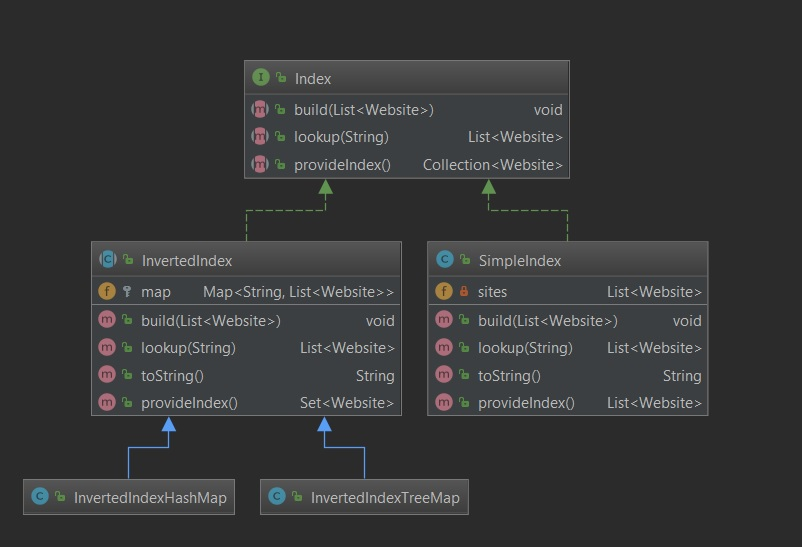
\includegraphics[width=\textwidth]{figures/Diagram_InvertedIndices}
    \caption{UML Diagram for the Software Architecture of Index data structures.}
    \label{fig:Index:uml}
\end{figure}

\subsection{FileHelper}
As part of the set up of this task, the {\tt FileHelper} class - specifically the \\ {\tt parseFile(String filename)} method – was updated such that from the database file, only websites that have a url, title, and at least one word of webpage content are read-in and stored in the server.
This was accomplished by an {\tt if} statements to check the assignments of the url and title fields prior to adding a {\tt new Website} object to the {\tt ArrayList<Website>}. However, the meat of the changes made to this method were to how the method recognised the content of each line scanned in in order to know how to treat it.
Previously, this was accomplished by making use of the knowledge of the very specific file format, {\tt String} methods, and {\tt boolean} field variables.
This was all replaced by two regular expressions:

{\tt Pattern website = Pattern.compile("(https?://[A-Za-z0-9./\_]+)");} \\
{\tt Pattern webTitle = Pattern.compile("[A-Z][a-z]+[A-Za-z0-9\textbackslash s]+?");} \\

and the methods of the {\tt Matcher} class. Though it does not look to be that big of a change, doing so means that the two field variables are no longer needed, hence less has to be juggled when reading and making further changes to the code.

\subsection{SimpleIndex}
The provided default way of storing indexes was called SimpleIndex. This solution is implemented using an ArrayList<website>, which contains all of the sites and each site than have their own ArrayList<String>  containing all the words on the sites. \\

\subsection{InvertedIndexTreeMap}
The second approach to store indexes was called InvertedIndexTreeMap. Here the relationship between site and it's words is inverted, meaning that each word knows to which sites it belongs to. The underlying data structure of the TreeMap is a Red-Black tree based NavigableMap implementation, sorted either by the natural ordering of its keys or by a Comparator. TreeMap provides \textit{guaranteed log(n) time} performance for the operations \textbf{containsKey, get, put, remove}.\cite{oracle:treemap} TreeMap use only the amount of memory needed to hold it's items, therefore this solution is suited when it is not known how many items have to be sorted in memory and there are memory limitations. Solutions is also suited when the order in which items have been stored is important and O(log n) search time is acceptable. \cite{baeldung:HashTreeCompared}

\subsection{InvertedIndexHashMap}
The third approach to store indexes was called InvertedIndexHashMap. Also in the HashMap the relationship between the site and it's words is inverted. To accomplish this a HashMap was used, where the words were used as Keys and  a List of websites as a Value.
The underlying data structure of the HashMap is a Hash table based implementation. This implementation gives \textit{constant-time} performance for the basic operations such as \textbf{get} and \textbf{put}. \cite{oracle:hashmap} However this is true under assumption that there are not too many collisions. This is because this Map implementation acts as a basket hash table and when buckets get too large, they get transformed into node of TreeNodes, similar to those in TreeMap. \cite{baeldung:HashTreeCompared} Some of the downsides of building the HashMap are that it requires more memory than it is necessary to hold its data and when a HashMap becomes full, it gets resized and rehashed, which is costly. HashMap solutions should be chosen in cases when the approximate amount of items have to be maintained in the collection is known and the order in which items have been stored is not important. \cite{baeldung:HashTreeCompared}


\section{Benchmarking}

In order to choose one of the implementations, namely ArrayList, TreeMap or HashMap, for the Search Engine, the benchmark test was performed to gain empirical data of the performance of each of the implementations. For the benchmark test, JMH (a Java harness for building, running, and analysing nano/micro/milli/macro benchmarks) was used. {OpenJDK:jmh} The benchmark test was carried out using 20 words (random nouns, verbs, adjectives and conjunctions), which were looked-up using the three different index implementations and in three different size databases: enwiki-tiny, enwiki-small, enwiki-medium. JMH provides information about an average Score, measured in nanoseconds per operation, the results of which can be found in table \ref{table:result}\\
During the benchmark it was assured that the test environment is as similar as possible among the different trials, meaning that all tests were performed on the same machine and no other applications running on the background.

\begin{table}[!htbp]
    \caption{\textbf{Benchmark Scores. Each score is an average in ns/op}}
    \begin{tabular}{|p{75pt}|p{75pt}|p{75pt}|p{75pt}|}
        \hline
        \textbf{Data sets} & \textbf{Simple} & \textbf{HashMap} & \textbf{Treemap} \\ \hline
        enwiki-tiny & 18944.884 & 1052.067 & 1591.311 \\ \hline
        enwiki-small & 8819338.592 & 1883.776 & 3622.582 \\ \hline
        enwiki-medium & 233498546.571 & 27451.020 & 30176.993 \\ \hline
    \end{tabular}
    \label{table:result}
\end{table}


The benchmark results shows that the SimpleIndex is significantly slower than both of the Inverted Map implementations: 233498546.571 ns/op versus 27451.020 ns/op for the InvertedIndexHashMap and 30176.993 ns/op for the InvertedIndexTreeMap using the enwiki-medium dataset.
In order to describe the results, let the number of websites be m and words be n.
The difference in performance can be explained as follows: \\
When the {\tt SimpleIndex} is looking up the search word, it looks though all the sites, which takes \textit{O(m)} time, and for each site it looks through all the words which takes \textit{O(n)} time, therefore total search time is \textit{O($m\cdot n$)}. The two other methods provide faster performance time. InvertedIndexTreeMap provides a \textit{guaranteed} performance of \textit{O(log(n))}. InvertedIndexTreeMap provides best-case performance of constant time \textit{O(1)} and the worst-case performance of \textit{O(log(n))} time (since Java 8). Worst-case performance occurs when the hash function is not implemented correctly and values are distributed poorly in buckets, leading to high hash collision.

%$2 \cdot log(n) + occ$\
There are several considerations when choosing the implementation for storing the data for the Search Engine.

HashMap seams to be better fit than a TreeMap for Search Engine solution, because in this case the order of data is not important whereas the performance looking up the websites corresponding the search word is. The HashMap can be expected to perform in constant time which is better than TreeMap's \textit{log(n)} time, and only in the HashMap's worst-case performance is it \textit{log(n)} time. The given data sets are fixed, therefore the costly resizing and rehashing is not going to occur implementing Hashmap. HashMap performed the best on all of the given different size datasets in benchmark test. This is the reasoning for choosing HashMap implementation over the TreeMap implementation for this Search Engine project.




\section{Testing Considerations}
After the above changes were implemented, development tests were written in order determine the viability of the code and whether the changes satisfied the requirements of the task. To that end, JUnit tests were devised for each class that was updated.

\subsubsection{FileHelper tests}
White-box tests were developed around the branching statements in the updated method, and a coverage table was produced,
please refer to Appendix \ref{tab:Coverage}. From this coverage table the  \ref{tab:Expectancy} was produced. The data
set data/test-file1.txt is an empty file, and the rest contained the data shown in \ref{tab:DataFiles}. This proccess
using the Coverage and Expectancy table shown in Appendix \ref{app:table}, is an example of how we construct our tests.

JUnit tests were then produced from table \ref{tab:Expectancy}, as found in FileHelperTest.java. Correctness was verfied along two axes: the size of
the {\tt List<Website>} returned, and the specific contents of the {\tt List}. As you can see from the Actual Output column of \ref{tab:Expectancy},
the updated code failed test B3, highlighting a weakness in the code, and subsequently had to be debugged. Including another IF statement after
the while loop resolved the issue, and following that all tests were passed.

\subsubsection{Index tests}
The correctness of the {\tt build} and {\tt lookUp} method were verified using unit tests (JUnit 5), which can be found in the {\tt IndexTest} file.
When setting up the test, a small {\tt List<Website>} was created which made it easier to predict the expected results of the methods. Each test
checks all of the indices using the white-box coverage considerations. The {\tt SimpleIndex} were more used as a reference to the others, and the
tests as it should be able to pass all test, due its simple nature.

The {\tt build} method was verified by creating a {\tt String} of what was expected the index should contain and then calling the {\tt toString} on
the index.

The {\tt lookUp} method was tested by providing it with words and then checking the size of the list returned against the expected size of that list.

Lastly, a test of checking whether the websites contained in the Index is the same as the websites read by the {\tt FileHelper} class was done.
This was performed on the tiny, small and medium files and was meant to see whether the behaviour of the index would stay the same when the
database size changed.

%How to reference surce\footnotemark. 
%\footnotetext{Oracle \url{https://docs.oracle.com/javase/8/docs/api/java/util/HashMap.html}} 

%How to reference surce\footnotemark. 
%\footnotetext{Oracle \url{https://docs.oracle.com/javase/8/docs/api/java/util/TreeMap.html}} 